\documentclass[12pt, a4paper]{article}
\usepackage[utf8]{inputenc}
\usepackage{indentfirst} %indentace prvního odstavce
\usepackage{mathtools}
\usepackage{amsfonts}
\usepackage{amsmath}
\usepackage{amssymb}
\usepackage{graphicx}

\graphicspath{{images/}}

\begin{document}


\section{}
Registr je délky 4 a jsme nad $\mathbb{Z}_2$, takže nabývá $2^4$ různých stavů.\\
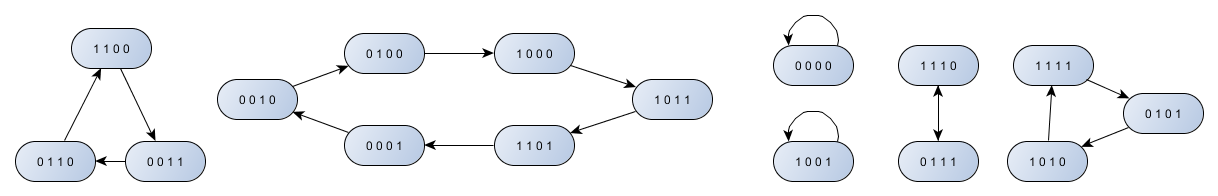
\includegraphics[width=\textwidth]{graf}

\section{}
Známe tedy i schéma v Galoisově tvaru, takže stačí dopočítat vnitřní stavy ($x_0, \dots, x_4$). Víme, že prvních 5 bitů výstupu jsou $11111$. Vždy se tedy k počátečním stavům přičte jednička při posunu nebo ne. Máme tedy rovnice:
$$s_0 = 1 = x_0 \Rightarrow x_0 = 1$$
$$s_1 = 1 = x_1 + 1 \Rightarrow x_1 = 0$$
$$s_2 = 1 = x_2 + 1 \Rightarrow x_2 = 0$$
$$s_3 = 1 = x_3 + 1 + 1 \Rightarrow x_3 = 1$$
$$s_4 = 1 = x_4 + 1 + 1 + 1 \Rightarrow x_4 = 0$$
Počáteční stav v Galoisově módu tedy je $10010$. $x^5+x^4+x^2+x+1$ je sice ireducibilní nad $\mathbb{Z}_2$ ale 1 (primitivní prvek $\mathbb{Z}_2$) není kořenem, takže nemůžeme použít větu. Každopádně po implementaci registru zjistíme, že perioda je stejně ta největší možná a to $2^5-1=31$.

\section{}
Pokud je $x_1 = 0$, tak výsledek odpovídá součinu $x_2 \cdot x_3$. Pokud je $x_1 = 1$, tak výsledek odpovídá skoro (až na poslední řádek, ale to se opraví přičtením již zjistěného $x_2 \cdot x_3$) součtu $x_2+x_3$, takže kandidátem na polynom je $x_1 \cdot (x_2+x_3) + x_2 \cdot x_3 = x_1 \cdot x_2 + x_1 \cdot x_3 + x_2 \cdot x_3$ a ten funguje.

\section{}
Pokud budeme uvažovat registr ve Fibonacciho tvaru, tak ze zadání známe $s_0 = 1, s_1 = 1, \cdots, s_9 = 1$. To co neznáme jsou koeficienty $c_0$ (ten je asi vždy 1) $, c_1, \cdots, c_4$. Dokážeme je ale dopočítat jednoduchou soustavou rovnic plynoucí ze schématu Fibonacciho registru. Např. $s_5 = s_0 \cdot c_0 + s_1 \cdot c_1 + s_2 \cdot c_2 + s_3 \cdot c_3 + s_4 \cdot c_4$. Dostaneme tedy soustavu rovnic:
$$
\begin{pmatrix}
s_0 & s_1 & s_2 & s_3 & s_4\\
s_1 & s_2 & s_3 & s_4 & s_5\\
s_2 & s_3 & s_4 & s_5 & s_6\\
s_3 & s_4 & s_5 & s_6 & s_7\\
s_4 & s_5 & s_6 & s_7 & s_8
\end{pmatrix}
\cdot
\begin{pmatrix}
c_0\\
c_1\\
c_2\\
c_3\\
c_4
\end{pmatrix}
=
\begin{pmatrix}
s_5\\
s_6\\
s_7\\
s_8\\
s_9
\end{pmatrix}
$$
$$
\begin{pmatrix}
1 & 1 & 1 & 1 & 1\\
1 & 1 & 1 & 1 & 0\\
1 & 1 & 1 & 0 & 0\\
1 & 1 & 0 & 0 & 0\\
1 & 0 & 0 & 0 & 1\\
\end{pmatrix}
\cdot
\begin{pmatrix}
c_0\\
c_1\\
c_2\\
c_3\\
c_4
\end{pmatrix}
=
\begin{pmatrix}
0\\
0\\
0\\
1\\
1
\end{pmatrix}
\Rightarrow
\begin{pmatrix}
c_0\\
c_1\\
c_2\\
c_3\\
c_4
\end{pmatrix} = \begin{pmatrix}
1\\
0\\
1\\
0\\
0
\end{pmatrix}
$$
Takže víme jak registr vypadá, naplníme ho stavem $s_0=0, \cdots, s_4=1$ a dopočítáme posloupnost. Prvních 10 bitů je: $0000100101$.

\section{}
Uvažujme registr v Galoisově tvaru. Poslední bit stavu je vždy výstupní bit předchozího stavu, je-li $c_0 = 1$, tak máme rovnost $a_0^{t+1} = a_{n-1}^{(t)} \cdot a_0$ pokud uvažujeme notaci z přednášky ($g = a$ a také $c = a$) viz obrázek:
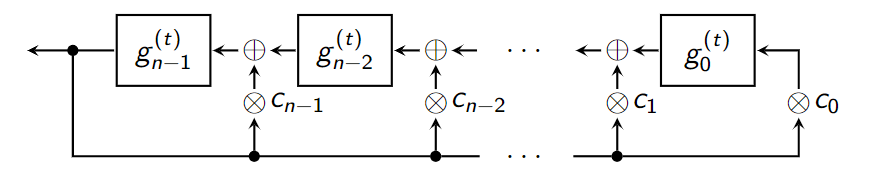
\includegraphics[width=\textwidth]{schema.png}
Dostaneme zase soustavu rovnic pro $L(a^{(t)}) = a^{(t+1)}$:
$$
\begin{pmatrix}
0 & 0 & 0 & \cdots & 0 & a_0\\
1 & 0 & 0 & \cdots & 0 & a_1\\
0 & 1 & 0 & \cdots & 0 & a_2 &\\
\vdots & \vdots & \ddots & \ddots & \vdots & \vdots \\
0 & 0 & \cdots & 1 & 0 & a_{n-2}\\
0 & 0 & \cdots & 0 & 1 & a_{n-1}\\
\end{pmatrix}
\cdot
\begin{pmatrix}
a_0^{(t)}\\
a_1^{(t)}\\
a_2^{(t)}\\
\vdots\\
a_{n-2}^{(t)}\\
a_{n-1}^{(t)}\\
\end{pmatrix}
=
\begin{pmatrix}
a_0^{(t+1)}\\
a_1^{(t+1)}\\
a_2^{(t+1)}\\
\vdots\\
a_{n-2}^{(t+1)}\\
a_{n-1}^{(t+1)}\\
\end{pmatrix}
$$
Inverzní matice existuje pouze v případě, pokud $a_0 \neq 0$ (jinak se dělí 0). V tomto případě vypadá $L^{-1}:$
$$
\begin{pmatrix}
a_1 & 1 & 0 & \cdots & 0 & 0\\
a_2 & 0 & 1 & \cdots & 0 & 0\\
a_3 & 0 & 0 & \ddots & 0 & 0 &\\
\vdots & \vdots & \ddots & \ddots & \vdots & \vdots \\
a_{n-1} & 0 & \cdots & 0 & 0 & 1\\
1 & 0 & \cdots & 0 & 0 & 0\\
\end{pmatrix}
$$

\section{}
Zadání 34. Jediné stavy v čase $t-2$, které přicházejí v úvahu jsou 2. První nastal tak, že se v čase $t-1$ posunuly registry R1, R2 a poté v čase $t-2$ také registry R1, R2. Druhý je také získaný posunitím R1, R2 v čase $t-1$ a v $t-2$ posunutím všech registrů.

Máme tedy 2 kandidáty. Zkontrolováním možných stavů v čase $t-3$ zjistíme, že jediný, který připadá v úvahu, je ten druhý. V čase $t-1$ se posunuly registry R1, R2 a v čase $t-2$ všechny 3. Stavy:
$$R1 = 0111011111111111010$$
$$R2 = 1100101100011011011011$$
$$R3 = 01111111011010000100101$$
\end{document}